% Author: Dr. Michael Ebner, Michael@DrEbner.net
% Date: May 2005

\documentclass[11pt,a4paper]{scrartcl}
\usepackage{setspace} 
\usepackage{geometry} 
\usepackage{hyperref}
\geometry{a4paper,tmargin=30mm,bmargin=30mm,lmargin=30mm,rmargin=30mm}
\usepackage[ngerman]{babel}

\usepackage[T1]{fontenc}      % T1-encoded fonts: auch Wörter mit Umlauten trennen
\usepackage[latin1]{inputenc}
\usepackage{currvita}

\usepackage{relsize}
\usepackage{soul}
\usepackage{xspace}


\usepackage[final]{graphicx}  % um Graphiken einzubinden
\usepackage{picins} %fuer bild einfuegen


\newcommand{\ccplusplus}{{\sffamily\smaller C/{C}\hbox{\kern.05em\raise.25ex%
  \hbox{+\kern-.01em+}\kern.05em}\spacefactor=1000 }}
\newcommand{\versal}[1]{\textsf{\textsmaller{\MakeUppercase{\caps{#1}}}}\xspace}

\newcommand*{\ac}[1]{\versal{#1}}
\tolerance=600

\renewcommand{\labelitemi}{$-$}
\renewcommand{\labelitemii}{$\bullet$}

\begin{document}
\parpic[rs][]{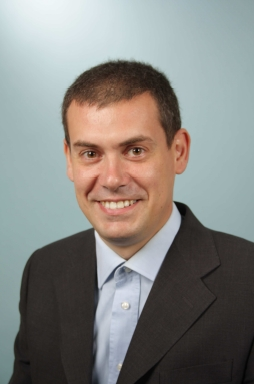
\includegraphics[width=3cm]{Profilfoto.jpg}}
\begin{cv}{Lebenslauf}
  \begin{cvlist}{Pers"onliche Daten}
  \item Dr. Michele Viti\\
    Kirchenstra{\ss}e 9\\
    22869 Schenefeld
  \item Telefon: 040 53273453\\
    Mobil: 0163 1903077\\
    E"~Mail:~micheleviti78@hotmail.com
  \item Geburtsdatum: 17.\,April\,1978\\
    Geburtsort: Arezzo, Italien\\
    Staatsangeh\"origkeit: italienisch
  \end{cvlist}
  
  \begin{cvlist}{Berufserfahrung}

  \item[06.2012-heute] Deutsches Elektronen-Synchrotron DESY Hamburg,
    R{\"o}ntgenstrahl-Detektoren Gruppe, Post-Doktorand\\

    Aufgaben:\\
    
    Teilnahme am Projekt PERCIVAL. Entwicklung eines neuen 
    bildgebenden CMOS-Detektors
    \begin{itemize}
    \item Teilnahme an Testmessungen
    \item Entwicklung des Softwareframeworks f{\"u}r Daten- und
      Bilderverarbeitung 
    \item Entwicklung einer graphischen Benutzerschnittstelle f{\"u}r  das Softwareframework
    \item Entwicklung der Software f{\"u}r das Data Acquisition
      System
    \item Entwicklung einer graphischen Benutzerschnittstelle mit Online
      Monitor f{\"u}r das Data Acquisition System
    \item Entwicklung der Software f{\"u}r die Auswertung der Testdaten
    \item ADC Charakterisierung und Kalibration
    \item Bestimmung der Detektoraufl{\"o}sung 
    \end{itemize}
      
      {\scshape {\bfseries Software:}}
      \begin{description} 
      \item[Betriebssysteme] : Ubuntu Linux, Scientific Linux, Windows
        XP/7
      \item[Programmiersprachen] : C++
      \item[Software framework] : Qt (Version 4.6.2 und 4.8.6)
      \item[Bibliotek] : Minuit
      \item[Datenanalyse] : ROOT
      \end{description}
    
  \item[01.2010-05.2012] Deutsches Elektronen-Synchrotron DESY
    Hamburg, ALFA Projekt des ATLAS Esperiments am CERN (Genf,
    Schweiz), Post-Doktorand \\
    
    Aufgaben:\\
    
    Im ALFA Projekt werden Spurdetektoren aus szintillierenden Fasern
    in beweglichen Vakuumtanks entlang der Strahlr{\"o}hre des LHC
    Beschleunigers installiert
    \begin{itemize}
    \item Vor der Installation der Detektoren im LHC Tunnel, Teilnahme
      an der Planung und der Durchf{\"u}hrung von Testmessung am CERN
      \begin{itemize}
      \item Rekonstruktion der Referenzspuren mit EUDET Silikon-Pixel
        Detektor und Durchf{\"u}hrung der Ausrichtung zwischen EUDET
        und ALFA Detektoren 
      \item Prozessierung der gesamten Daten der Testmessung mit den
        selbstentwickelten Programmen und Vorbereitung f{\"u}r die
        Auswertung innerhalb der ALFA Gruppe
      \item Beteligung an der Testdatenanalyse
      \end{itemize}           
    \item Anfang 2011 Installation der Detektoren abgeschlossen
      \begin{itemize}
      \item Zur Zeit Koordinator der "`Data Preparation"'-Gruppe, die
        f{\"u}r die Aufbereitung und Prozessierung der Daten f{\"u}r
        die Physikanalyse verantwortlich ist
      \item Beteiligung an der physikalischen Datenanalyse
      \item Pflege und weitere Entwicklung von Softwareschnittstellen
      \end{itemize} 
    \end{itemize}

    {\scshape {\bfseries Software:}}
    \begin{description} 
    \item[Betriebssysteme] : Ubuntu Linux, Scientific Linux, Windows
      XP/7
    \item[Programmiersprachen] : C++, Python
    \item[Software framework] : Marlin
    \item[Bibliotek] : Minuit
    \item[Datenanalyse] : ROOT
    \end{description}
    
  \item[02.2006-12.2009] Deutsches Elektronen-Synchrotron DESY Zeuthen,
    International Linear Collider Projekt, Wissenschaftlicher Mitarbeiter \\
    
    Aufgaben:\\
    
    Siehe Doktorarbeit.
    
  \item[02.2005-01.2006] Perugia
    Universit\"at, Italien, wissenschaftlicher Mitarbeiter \\
    
    Aufgaben:\\
    
    Fortsetzung der Diplomarbeit.
    
  \end{cvlist}
  
  \begin{cvlist}{Promotion}
  \item[02.2006-08.2009] 
    
    Deutsches Elektronen-Synchrotron DESY, Zeuthen, Linear Collider
    Gruppe, Doktorand / wissenschaftlicher Mitarbeiter\\ Thema:
    "`Precise and Fast Beam Energy Measurements at the International
    Linear Collider"'

    Aufgaben:\\ 
    
    \begin{itemize}
      
    \item Test und Bau eines Prototyps f{\"u}r die
      Strahlenergiemessung einer zuk{\"u}nftigen
      Teilchenbeschleunigermaschine am Stanford Accelerator Center in
      der USA
      \begin{itemize}
      \item Teilnahme an der Planung, Durchf{\"u}hrung und der
        Datenaufnahme des Tests
      \item Test der Dipolmagnete des Apparates.
      \item Messdatenauswertung und Bestimmung der Aufl{\"o}sung der
        Strahlenergiemessung
      \end{itemize}
      
    \item Machbarkeitsstudie einer neuen Methode f{\"u}r die
      Strahlenergiemessung, die auf Comptonstreuung von
      Strahlteilchen mit Laserphotonen beruht
      \begin{itemize}
      \item Simulation des Layouts des Prototyps.
      \item Untersuchung der Anforderungen f{\"u}r die
        Lasereigenschaften
      \item Simulation und Untersuchung f{\"u}r verschiedene
        Detektoren
      \item Berechnung und Sch{\"a}tzung von physikalischen
        Hintergrundprozessen und deren Wirkung auf die
        Strahlenergiemessung
      \end{itemize}
      
    \end{itemize}
    
    {\scshape {\bfseries Software:}}
    \begin{description} 
    \item[Betriebssysteme] : Ubuntu Linux, Scientific Linux, Windows XP
    \item[Programmiersprachen] : C++, Python, Fotran
    \item[Software framework] : GEANT 4
    \item[Bibliotek] : Minuit
    \item[Datenanalyse] : ROOT
    \item[Monte Carlo Generator] : CAIN, COMRAD
    \end{description}
    
  \item[11.2009] Verteidigung der Doktorarbeit
    
  \end{cvlist}
  
  \begin{cvlist}{Studium}
  \item [11.1997-10.2004]Perugia Universit\"at, Italien, Physik
    Studium. \\ Schwerpunkt: Teilchenphysik\\ Abschluss: Diplom
    Physik, Thema der Diplomarbeit: "`Evaluation of a Tracking
    Algorithm for the Trigger of the KOPIO Experiment on the Decay
    $K_L^0\rightarrow\pi^0\nu\bar{\nu}$"'\\
    
    Aufgaben:\\
    
    \begin{itemize}	
    \item Simulation eines Mustererkennungsalgorithmus (Pattern
      Recognition) f{\"u}r den Trigger des KOPIO Experiments
    \item Entwicklung eines Event Display f{\"u}r das Simulationsprogramm
    \end{itemize}
    
    {\scshape {\bfseries Software:}}
    \begin{description} 
    \item[Betriebssysteme] : Windows XP, Red Hat Linux 
    \item[Programmiersprachen] : Fortran, C 
    \item[Software framework] : GEANT 3
    \item[Bibliotek] : OpenGL
    \item[Datenanalyse] : PAW
    \end{description}
  \end{cvlist}

  \begin{cvlist}{Schulabschluss}
  \item[07.1997] Wissenschaftliches Gymnasium Liceo Scientifico "`G. da
    Castiglione"', Castiglion Fiorentino, Italien
  \end{cvlist}
  
  \begin{cvlist}{F\"uhrungspositionen}
  \item [07.2011-heute] Koordinator der "`Data Preparation"'-Gruppe
    f\"ur das ALFA Projekt
    %\begin{cvlist}{Weitere Qualifikationen}
    %\item[06.2008] Specialized CERN Accelerator School "Beam Diagnostics", Dourdan, Frankreich
    %\item[09.2010] Workshop ``Advanced Methods of Software Development'', Dresden
  \end{cvlist}

  \begin{cvlist}{Lehre}
  \item [07.2006-09.2006] Betreuung von DESY-Sommerstudent
  \item [07.2007-09.2007] Betreuung von DESY-Sommerstudent
  \item [07.2010-09.2010] Betreuung von DESY-Sommerstudent
  \item [04.2011-02.2012] Betreuung von Masterstudent
  \end{cvlist}
  
  \begin{cvlist}{Berufliche Auslandsaufenthalte}
  \item [02.2006-heute] Leben und arbeiten in Deutschland
  \item [2006-2007] 5 Aufenthaltsperioden in Stanford Universit\"at, USA.
  \item [02.2008] Nowosibirsk, Russische F\"oderation
  \item [01.2010-heute] Regelm\"a{\ss}ige Aufenthalte in Genf, Schweiz
  \end{cvlist}

  \begin{cvlist}{Sprachkenntnisse}
  \item Italienisch: Muttersprache
  \item Deutsch: verhandlungssicher
  \item Englisch: verhandlungssicher
  \end{cvlist}

  \begin{cvlist}{Weitere \ac{EDV} Kenntnisse}
  \item[Programmiersprachen] Pascal, \ac{BASIC}
  \item[Sonstiges] \ac{MS OFFICE}, \ac{\LaTeX}, UML(Grundkenntnisse)
  \end{cvlist}
  
  %\begin{cvlist}{Internal Notes}
  %\item[] M.~Viti and S. Kostromin, Magnetic measurements for magnets
  %  10D37, ILC-SLACESA TN-2008-1, 2008
  %\end{cvlist}

  \begin{cvlist}{Freizeit}
  \item Segeln (SBF Binnen, SBF See, SKS)
  \item Vereinsmitglied "`Verein Jugendsegeln e.V."', Kiel
  \item Besatzungsmitglied des Traditionsseglers "`Pr\"asident Freiherr
    von Maltzahn"', Museumshafen \"Ovelg\"onne e.V., Hamburg
  \item Wandern
  \item Plattdeutsch
  \end{cvlist}

  %\begin{cvlist}{Publikationen}
  %\item M. Viti, Precise and fast beam energy measurement at the
  %  International Linear Collider, DESY-THESIS-2010-007
  %  %\item M. Viti, Precise and Fast Beam Energy Measurement: Studies on the
  %  % upstream beam energy monitors at the International Linear Collider,
  %  % Suedwestdeutscher Verlag fuer Hochschulschriften, Juni 2010
  %\item H.-J. Schreiber et al. (M.Viti) Magnetic measurements and simulations of
  %  a 4-magnet dipole chicane for the International Linear Collider,
  %  Particle Accelerator Conference (PAC07), Albuquerque, NM, U.S.A
  %\item M. Viti, Energy measurement with Compton backscattering:
  %  Updates, LCWS-2007-MDI23
  %\item N. Muchnoi, H. J. Schreiber and M. Viti, ILC beam energy
  %  measurement by means of laser Compton Backscattering,
  %  Nucl. Instrum. Meth., A607:340-366, 2009
  %\item A. Lyapin et al. (M.Viti) Results from a prototype chicane-based energy
  %  spectrometer for a linear collider JINST 6 (2011) P02002,
  %  arXiv:1011.0337
  %\item M. Viti, Forward Physics Results from ATLAS, Hadron Structure
  %  '11, Tatransk\'a \v{S}trba, Slovak Republic
  %\item ATLAS authorship
  %\end{cvlist}

  \cvplace{Hamburg}
  \date{27.~Marz~2014}

\end{cv}

\newpage

%\begin{center}
%  \huge{Publications List}
%\end{center}
%\vspace{1cm}
%       {\bfseries Talks, Poster Sessions and Proceedings}
%       \begin{itemize}
%       \item Dubna Beam Energy Measurement Workshop, Joint Institute for
%         Nuclear Research (JINR), Dubna, June 2006.
%       \item European Particle Accelerator Conference (EPAC 06), Edinburgh,
%         Scotland, 26-30 June 2006.
%       \item Yerevan Beam Energy Measurement Workshop, Yerevan Physics
%         Institute, Yerevan, October 2006.
%       \item DPG Fr\"uhjahrstagung, Heidelberg, 5-9 March 2007.
%       \item 2007 International Linear Collider Workshop (LCWS07 and ILC07),
%         Hamburg, Germany, 30 May - 3 June 2007.
%       \item Zeuthen Beam Energy Measurement Workshop, Zeuthen, June 2007,
%       \item Particle Accelerator Conference PAC07, Albuquerque, New Mexico,
%         25-29 June 2007.
%       \item DPG Fr\"uhjahrstagung, Freiburg, 3-7 March 2008.
%       \item Workshop on Polarization and Beam Energy Measurements at the
%         ILC, Zeuthen, 9-11 April 2008.
%       \item ILC-ECFA Workshop, Warsaw, Poland, 9-12 June 2008.
%       \item EUDET Annual Meeting 2010, Hamburg, Germany, 29 September - 1 October 2010.
%       \item M. Viti, Forward Physics Results from ATLAS, Nuclear Physics B
%         (Proc. Suppl.) $219-220$ (2011) $145-148$.
%       \end{itemize}
%           {\bfseries Internal Notes}
%           \begin{itemize}
%           \item M. Viti and S. Kostromin, Magnetic measurements for magnets
%             10D37, ILC-SLACESA TN-2008-1, 2008.
%           \item B. Allongue et al. Results from the ALFA test beam campaign in
%             2009, ATL-COM-LUM-2010-031, CERN Geneva, October 2010.
%           \end{itemize}
%               {\bfseries Publications}
%               \begin{itemize} 
%               \item M. Viti, Precise and fast beam energy measurement at the
%                 International Linear Collider, DESY-THESIS-2010-007
%               \item N. Muchnoi, H. J. Schreiber and M. Viti, ILC beam energy
%                 measurement by means of laser Compton Backscattering,
%                 Nucl. Instrum. Meth., A607:340-366, 2009.
%               \item A. Lyapin et al. Results from a prototype chicane-based energy
%                 spectrometer for a linear collider JINST 6 (2011) P02002,
%                 arXiv:1011.0337
%               \item ATLAS authorship.
%               \end{itemize}

\end{document}
\endinput
%%
%% End of file
